%=========================================================================
% (c) Michal Bidlo, Bohuslav Křena, 2008

\chapter{Introduction}

...\\
...\\
...\\

\chapter{Relevant projects}

In this chapter describes BeakerLib and projects relevant to it.

\section{BeakerLib}

BeakerLib is a shell-level integration testing library, providing convenience functions which simplify writing, running and analysis of integration and blackbox tests. 
It is developed and maintained by Red Hat and operates under GNU General Public License.
\begin{itemize}
\item Main features of BeakerLib include:
\item Journal - uniform logging mechanism. 
\item Phases - logical grouping of test actions, clear separation of setup / test / cleanup
\item Asserts - common checks affecting the overall results of the individual phases (checking for exit codes, file existence \& content...)
\item Helpers - convenience functions for common operations such as managing services, backup \& restore 
\end{itemize}
[citace beakerlib github wiki]

This thesis focuses on BeakerLib Journal and problem it causes with long tests.


\section{Beaker}

Beaker is a full stack software and hardware integration testing system, with the ability to manage a globally distributed network of test labs.  [citace beaker doc] It is Red Hat community project under GNU General Public License version 2.

Main functionality includes management of hardware inventory, on which Beaker can install wide variety  of operating systems from Red Hat Linux family. Another notable part  is Task library which contains rpm packages of individual tests which can be run on provided machines. 
Users then can specify which hardware they require with which OS and tests they want to run on it through either command-line tools or web interface both of which are part of Beaker install package [link to beaker download page?]. If Beaker meets given criteria in its inventory it installs Test harness to which it gives list of tests to be run.  After Test Harness finishes running the tests, results are sent back to Beaker where they are stored for specified period of time. 

\subsection{beaker-wizard}
Part of Beaker package. Interactive command-line tool which automates creation of BeakerLib tests. Using predefined or user-defined templates it creates all files that are needed to run BeakerLib test.

\section{Test Harness}
Test harness is a software framework that automates test execution. It contains tests to be run, executes them and reports results. <expand>

Beaker’s harnesses prepare environment for BeakerLib by setting variables to proper values.

\subsection{Beah harness}
Default Beaker harness . <expand> [link to doc]

\subsection{Restraint harness}
Alternative Beaker harness which can, unlike Beah, run with Beaker or standalone without it. <expand> [link to doc]
\\
\\
Relations between Beaker, Harness and BeakerLib is shown in figure \ref{fig:beaker_relation}

\begin{figure}[h!]
  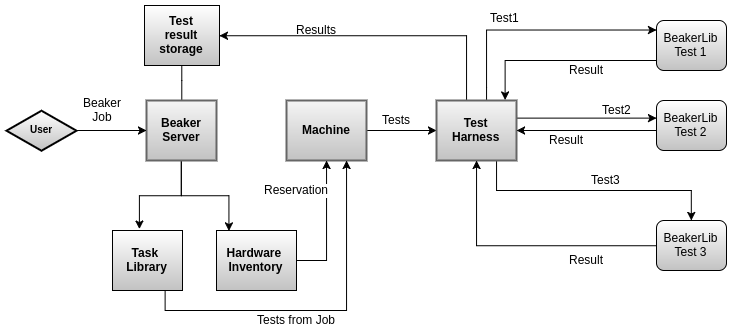
\includegraphics[width=\linewidth]{beaker_relations.png}
  \caption{Beaker relation to BeakerLib}
  \label{fig:beaker_relation}
\end{figure}




\chapter{BeakerLib}

\section{More in-depth description}

\section{Journal in-depth}

\section{Proposed solutions}

\subsection{Change of xml parser}

\subsection{Change in accessing journalling.py}

\subsubsection{Queue file solution}


\subsubsection{Daemon-like solution}



\chapter{Performance measuring}
<Definition of performance measuring>

For performance measuring of BeakerLib I chose two kinds of tests in in two kinds of testing environments.

\section{Tests}

\subsection{Artificial tests}
First type of tests are artificial tests created by me with beaker-wizard* to specifically target and measure performance of journalling modification I made. They consist mostly of commands that directly work with journalling.xml. For example commands rlLog or rlPhaseStart and rlPhaseEnd. That way we can observe clear difference in performance without being affected by operations unrelated to journalling (executing actions that verify functionality of components in real tests). 

<description of artificial tests with links to Appendix>

\subsection{Real tests}
Second type are real tests used in Red Hat. These are examples of tests that have been reported to have bad performance with BeakerLib so I am testing them to see if my modifications have real life impact on performance.

<description of real tests>

\section{Testing Environment}

\subsection{Local}
First environment is local laptop for convenience and speed of execution. I measured  two parameters, time of execution of each test and memory usage during execution. Tests were run directly, without any harness and with these technical specifications. 

<table of tech specs>

\subsection{Remote in beaker}
Second round of testing was done to emulate real testing conditions. I created Beaker recipe containing all performance tests which I submitted to Red Hat beaker server. Only time of execution was measured in remote testing.

<table of tech specs>

\section{Baseline measurements}
<results>


\section{Implemented optimizations}
<results>

\chapter{Conclusion}
Recap of results
\\
Future work

%=========================================================================
